\pdfminorversion=4
\documentclass[12pt]{article}

%\usepackage{geometry} % see geometry.pdf on how to lay out the page. There's lots.
%\geometry{a4paper} % or letter or a5paper or ... etc
% \geometry{landscape} % rotated page geometry

\usepackage[textwidth = 6in, textheight = 8.5in]{geometry}
% \geometry{
% a4paper
% }

%\usepackage{fontspec}
%\setmainfont{Times New Roman}

% For general mathematical display:
\usepackage{amsthm}
\usepackage{amssymb}
\usepackage{amsmath}
\usepackage{bm}
\usepackage{amsbsy}
\usepackage{bigints} % Control the size of integral symbols.
\usepackage{relsize}
\usepackage{mathrsfs}
\usepackage{mathtools}
\usepackage{accents}
\usepackage{enumitem}
\usepackage{amsfonts}
%\usepackage{paralist}
\allowdisplaybreaks

% For referencing an external document:
\usepackage{xr}
\externaldocument{app}

% New commands and operators:
\def\sigsqeps{\sigma^2_{\epsilon}}
\def\aeps{a_{\epsilon}}
\def\Asqeps{A_{\epsilon}^2}
\def\Sigmanu{\bSigma_{\nu}}
\def\munu{\bmu_{\nu}}
\def\sigsqmu{\sigma^2_{\mu}}
\def\amu{a_{\mu}}
\def\Asqmu{A_{\mu}^2}
\def\const{\text{const.}}
\def\rest{\text{rest}}
\def\mumu{\bmu_\mu}
\def\betamu{\bbeta_\mu}
\def\umu{\bu_\mu}
\def\numu{\bnu_\mu}
\def\Vpsi{\bV_\psi}
\newcommand{\sigsqb}[1]{\sigma^2_{b_{#1}}}
\newcommand{\ab}[1]{a_{b_{#1}}}
\newcommand\betapsi[1]{\bbeta_{\psi_{#1}}}
\newcommand\upsi[1]{\bu_{\psi_{#1}}}
\newcommand\nupsi[1]{\bnu_{\psi_{#1}}}
\newcommand\sigsqpsi[1]{\sigma^2_{\psi_{#1}}}
\newcommand\apsi[1]{a_{\psi_{#1}}}
\newcommand\Asqpsi[1]{A_{\psi_{#1}}^2}
\newcommand\hmu[1]{h_{\mu, i}}
\newcommand\hmupsi[1]{\bh_{\mu \psi, i}}
\newcommand\Hpsi[1]{\bH_{\psi, i}}
\newcommand\mupsi[1]{\bmu_{\psi_#1}}
\newcommand\tni[1]{\text{terms not involving $#1$}}

% Linespacing:
\usepackage{setspace}
%\singlespacing
%\onehalfspacing
\doublespacing

% Let top 85% of a page contain a figure
\renewcommand{\topfraction}{0.85}

% Default amount of minimum text on page (Set to 10%)
\renewcommand{\textfraction}{0.1}

% Only place figures by themselves if they take up more than 75% of the page
\renewcommand{\floatpagefraction}{0.75}

% For chapter quotes:
\usepackage{epigraph}

% For author list:
\usepackage[T1]{fontenc}
\usepackage[utf8]{inputenc}
\usepackage{authblk}

% For theorems and so on:
\usepackage[english]{babel}
\makeatletter
\def\thmhead@plain#1#2#3{%
  \thmname{#1}\thmnumber{\@ifnotempty{#1}{ }\@upn{#2}}%
  \thmnote{ {\the\thm@notefont#3}}}
\let\thmhead\thmhead@plain
\makeatother

\theoremstyle{plain}
\newtheorem{theorem}{Theorem}[section]
\newtheorem{lemma}[theorem]{Lemma}
\newtheorem{proposition}[theorem]{Proposition}
\newtheorem{result}{Result}[section]
\newtheorem{corollary}[theorem]{Corollary}
\newtheorem{claim}[theorem]{Claim}
\newtheorem{assumption}{Assumption}

\theoremstyle{definition}
\newtheorem{definition}{Definition}[section]
\newtheorem{conjecture}{Conjecture}[section]
\newtheorem{example}{Example}[section]

\theoremstyle{remark}
\newtheorem*{remark}{Remark}
\newtheorem*{note}{Note}

% For creating figures, tables and drawing graphs:
\usepackage[font={small}]{caption}
\usepackage{graphicx}
\usepackage{subcaption}
\usepackage{cleveref}
\usepackage[labelformat=simple]{subcaption}
\renewcommand\thesubfigure{(\alph{subfigure})}
\usepackage{tikz}
\usetikzlibrary{arrows,positioning,calc,fit}
\usetikzlibrary{shapes.geometric}
\usetikzlibrary{automata}
\usepackage{tkz-euclide}
\renewcommand{\arraystretch}{1} % Adjust value for vertical spacing in tables
\usepackage[bottom]{footmisc} % Keeps floats above footnotes
\usepackage{booktabs}
\usepackage{siunitx}
\usepackage{tabularx}
\usepackage{colortbl}
\usepackage{rotating}
\usepackage{tcolorbox}
\usepackage{pgffor}

% For adding to do notes:
\usepackage{xcolor}
\newcommand\extra[1]{\textcolor{red}{#1}}

% For Bibliography:
\usepackage{cite}
\usepackage{pslatex,apacite} 
\bibliographystyle{apacite}

% For Appendices:
\usepackage{etoolbox}
\pretocmd{\chapter}{\renewcommand\thesection{\thechapter.\arabic{section}}}{}{}
\newcommand\appsection{%
  \setcounter{section}{0}%
  \renewcommand\thesection{\thechapter.\Alph{section}}}

% For macros:
\usepackage{import}
\import{}{macros}

% For choosing which chapter to compile:
%\includeonly{Introduction, VariationalBayesianInference}

% For hyphenating words that may break the right-hand margin:

% See the ``Article customise'' template for some common customisations

\newif\ifblinded

\blindedfalse

\ifblinded
	
	\title{Bayesian Functional Principal Components Analysis via Variational Message Passing}
	\author{}
	
\else
	
	\title{Bayesian Functional Principal Components Analysis via Variational Message Passing}
	\author[1,2,3]{Tui H. Nolan \thanks{Corresponding author: tn352@cam.ac.uk}}
	\author[4]{Jeff Goldsmith}
	\author[1,5]{David Ruppert}
	\affil[1]{School of Operations Research and Information Engineering, Cornell University}
	\affil[2]{Medical Research Council Biostatistics Unit, The University of Cambridge}
	\affil[3]{School of Mathematical and Physical Sciences, University of Technology Sydney}
	\affil[4]{Department of Biostatistics, Mailman School of Public Health, Columbia University}
	\affil[5]{Department of Statistics and Data Science, Cornell University}
	
\fi

%%% BEGIN DOCUMENT
\begin{document}

\maketitle

\section*{\centering Abstract}

Standard approaches for functional principal components analysis
rely on an eigendecomposition of a smoothed covariance surface in order to extract the orthonormal eigenfunctions
representing the major modes of variation in a set of functional data.
This approach can be a computationally intensive procedure, especially
in the presence of large datasets with irregular observations. In this article, we develop a variational Bayesian approach,
which aims to determine the Karhunen-Lo\`{e}ve decomposition directly without smoothing and estimating a
covariance surface. More specifically, we incorporate the notion of variational message passing over a factor graph 
because it removes the need for rederiving approximate
posterior density functions if there is a change in the model. Instead, model changes are handled by changing
specific computational units, known as fragments, within the factor graph. 
Indeed, this is the first article to address a functional data model
via variational message passing. Our approach introduces two new fragments that are necessary for Bayesian
functional principal components analysis. We present the computational details, a set of simulations for assessing the
accuracy and speed of the variational message passing algorithm and an application to United States temperature data.

\noindent \emph{Keywords:} nonparametric regression, Kullback-Liebler divergence, functional principal component scores

%%%%%%%%%%%%%%  INTRODUCTION  %%%%%%%%%%%%%%%

\section{Introduction}
\label{sec:intro}

Functional principal components analysis (FPCA) is the methodological extension of classical principal
components analysis (PCA) to functional data. Within the overarching framework of functional data analysis,
FPCA is a central technique. The advantages of using FPCA for functional data are derived
from analogous advantages that PCA affords for multivariate data analysis. For instance, PCA in the multivariate
data setting is used to reduce dimensionality and identify the major modes of variation of the
data set. The modes of variation are determined by the eigenvectors of the sample covariance matrix of the data
set, while dimension reduction is achieved by identifying the eigenvectors that maximize variation in the data.
In the functional setting, response curves are interpreted as independent realisations of an underlying
stochastic process. A covariance operator and its eigenfunctions play the analogous
role that the covariance matrix and its eigenvectors play in the multivariate data setting. By identifying the
eigenfunctions with the largest eigenvalues, one can reduce the
dimensionality of the entire data set by approximating each curve as a linear combination of the reduced set
of eigenfunctions.

There are technical issues that arise in the functional setting that are not present for multivariate data.
The domain of the functional curves is typically a compact interval $[0, T]$ of the real line.
Despite having a continuous domain, the curves are only observed at discrete points over this interval.
Furthermore, the points of observation, as well as the total number of observations, need not be the
same for each curve. Therefore, approaches that are used in PCA require
modifications to extend to the functional framework.
In FPCA, we often rely on nonparametric regression to smooth the eigenfunctions and employ
an appropriate step to ensure that they are orthonormal from the perspective of integration, rather
than inner products of vectors.

There have been numerous developments in FPCA methodology throughout the statistical literature.
A thorough introduction to the statistical framework and applications can be found in \citeA[Chapter~8]{ramsay05}
and \citeA[Section~2]{wang16}. Much of this work mirrors the eigendecomposition approach to PCA, in that an
eigenbasis is obtained from a covariance surface. \citeA{yao05} focused on the case of sparsely observed functional
data, and estimate
principal component scores through conditional expectations. \citeA{xiao16} developed a fast covariance estimation method for densely observed functional data. \citeA{di09} extended FPCA to multilevel functional data, extracting within and
between subject sources of variability, and \citeA{greven2011} developed methods for longitudinal functional data. However,
\citeA{goldsmith13} noted that these approaches implicitly condition on an estimated eigenbasis to estimate scores, meaning that inference on
individual curve estimates can be inaccurate.

Meanwhile, other approaches have built on or are similar to the probabilistic PCA framework that was introduced by \citeA{tipping99} and \citeA{bishop99}. Rather than first obtaining eigenfunctions from a covariance and then estimating scores, all quantities are considered unknown and are estimated jointly.  \citeA{james2000} used an expectation maximization algorithm for estimation and inference in the context of sparsely observed curves. Variational Bayes for FPCA was introduced by \citeA{vanderlinde08} via a generative model with a factorized approximation of the full posterior density function. \citeA{Goldsmith15} introduced a fully Bayes framework for multilevel function-on-scalar
regression models with FPCA applied to two levels of residuals,
and also considered observed values that arise from exponential family distributions. 

In frequentist versions of FPCA, the covariance function is determined through bivariate smoothing of the raw
covariances. Eigenfunctions and eigenvalues are then determined from the smoothed covariance function.
The key advantage in the Bayesian approach is that the covariance function is not estimated, meaning that
complex bivariate smoothing is not required. Indeed, the eigenfunctions and eigenvalues are computed directly
as part of a Bayesian hierarchical model. Furthermore, it is unnecessary to compute or store large covariance matrices for dense functional data, and for sparse, irregular functional data -- where estimating the raw covariance is difficult or impossible -- direct estimation of eigenfunctions in a Bayesian model is straightforward. For these reasons, we pursue a Bayesian approach to FPCA.

Although there have been numerous contributions to Bayesian implementations of FPCA, we argue that there are
additional considerations that should be addressed. First, MCMC modeling of FPCA is a computationally expensive
procedure and, in some biostatistical applications \cite{Goldsmith15}, the computational time can reach several
hours. Second, current versions of variational Bayes for FPCA, despite being a much faster computational alternative,
are difficult to extend to more complex likelihood specifications, such as multilevel data models and binary response
outcomes.

\citeA{minka05} presents a unifying view of approximate Bayesian inference under a message passing framework
that relies on the notion of messages passed between nodes of a factor graph. Mean field variational Bayes (MFVB)
\cite{ormerod10, blei17}
can be incorporated into this framework through an alternate scheme known as variational message passing (VMP)
\cite{winn05}. \citeA{wand17} introduced computational units, known as fragments, that compartmentalize
the algebraic derivations that are necessary for approximate Bayesian inference in VMP. The notion of fragments
within a factor graph is essential for efficient extensions of variational Bayes-based FPCA to arbitrarily large statistical
models.

In this article, we propose an FPCA extension of the VMP framework for variational Bayesian inference set out in
\citeA{wand17}. Our novel methodology includes the introduction of two fragments  that are necessary for
computing approximate posterior density functions under an MFVB scheme,
as well as a sequence of post-processing steps for estimating the orthonormal eigenfunctions.
Section \ref{sec:fpca} gives an overview of FPCA and
introduces the Bayesian hierarchical model.
We provide an introduction to
variational Bayesian inference in Section \ref{sec:vbi}, with an overview of VMP in Section \ref{sec:vmp}.
In Section \ref{sec:post_vmp_steps}, we outline the post-VMP steps that are required for
producing orthonormal eigenfunctions. Simulations, including speed and accuracy comparisons with MCMC
algorithms, are presented in Section \ref{sec:sims}, and an application to United States temperature data is
provided in Section \ref{sec:us_weather_data}.

%%%%%%%%%%%  FUNCTIONAL  PRINCIPAL  COMPONENTS  ANALYSIS  %%%%%%%%%%%

\section{Functional Principal Components Analysis}
\label{sec:fpca}

Consider a random sample of i.i.d.\ smooth random functions $y_1, \dots, y_n \in L^2 [0, 1]$. We will assume the
existence of a continuous mean function $\mu = \E y_i$ and continuous covariance surface
$\sigma (t, s) = \E [ \{ y_i (t) - \mu (t) \} \{ y_i (s) - \mu (s) \} ]$, $i = 1, \dots, n$.
Then, the covariance operator $\Sigma$ of $y_i$ is defined as $(\Sigma g) (t) \equiv \int_0^1 \sigma (t, s) g(s) ds$, 
$g \in L^2 [0, 1]$. From Mercer's Theorem, the spectral decomposition of $\Sigma$ satisfies $\sigma (s, t) =
\sum_{l=1}^\infty \gamma_l \ \psi^*_l (s) \ \psi^*_l (t)$, where the $\gamma_l$ are the eigenvalues of
$\Sigma$ in descending
order and $\psi^*_l$ are the corresponding orthonormal eigenfunctions. The Karhunen-Lo\`{e}ve decomposition
is the basis for the FPCA expansion \cite{yao05}:

\begin{equation}
	y_i (t) = \mu (t) + \sum_{l=1}^\infty \zeta^*_{il} \ \psi^*_l (t), \quad i = 1, \dots, n,
\label{kl_expansion}
\end{equation}

\noindent where $\zeta^*_{il} = \int_0^1 \{ y_i (t) - \mu(t) \} \psi^*_l(t) dt$ are the principal components
scores. The $\zeta^*_{il}$ are independent across $i$ and uncorrelated across $l$, with $\E (\zeta^*_{il}) = 0$
and $\Var (\zeta^*_{il}) = \gamma_l$. Note that under the Gaussian assumptions that we introduce  in
\eqref{bayes_fpca_mod}, the $\zeta^*_{il}$ are also independent across $l$.
The asterisk is used as a reminder that the eigenfunctions in
\eqref{kl_expansion} are orthonormal and that the scores are independent.

Expansion \eqref{kl_expansion} facilitates dimension reduction by providing a best approximation for each
curve $y_1, \dots, y_n$ in terms of the truncated sums involving the first $L$ orthonormal eigenfunctions
$\psi^*_1, \dots, \psi^*_L$. That is, for any choice of $L$ orthonormal eigenfunctions $\psi_1, \dots, \psi_L$, the
minimum of $\sum_{i=1}^n \left|\left| y_i - \mu - \sum_{l=1}^L \langle y_i - \mu , \psi_l \rangle \psi_l \right|\right|^2$
is achieved for $\psi_l = \psi^*_l$, $l = 1, \dots, L$, where $|| \cdot ||$ denotes the $L^2$ norm and
$\langle \cdot, \cdot \rangle$ denotes the $L^2$ inner product. For this reason, we define the best estimate of
$y_i$ as

\begin{equation}
	\yhat_i (t) \equiv \mu (t) + \sum_{l=1}^L \zeta^*_{il} \ \psi^*_l (t), \quad i = 1, \dots, n.
\label{yhat}
\end{equation}

For the remainder of this article, we assume that all eigenvalues of the covariance operator have multiplicity one.
In addition, issues of identifiability are always present when one attempts to infer eigenfunctions or eigenvectors.
However, choosing one eigenfunction over its opposite sign has no effect on the resulting fits, although one choice
of sign may provide more natural interpretation of the eigenfunction. Here, we simply assume that
the signs of the orthonormal eigenfunctions $\psi^*_1, \dots, \psi^*_L$ are such that if $\psihat_l$ is an
estimator of $\psi^*_l$, then $\langle \psi^*_l , \psihat_l \rangle > 0$.

Expansions similar to \eqref{yhat} are also possible, where

\begin{equation}
	\yhat_i (t) \equiv \mu (t) + \sum_{l=1}^L \zeta_{il} \ \psi_l (t), \quad i = 1, \dots, n,
\label{yhat_not_orthogonal}
\end{equation}

\noindent where $\zeta_{il}$ are correlated across $l$, but remain independent across $i$, and the $\psi_l$ are not
orthonormal. Theorem \ref{thm:orth_basis} shows that an orthogonal decomposition of the resulting basis functions
and scores is sufficient for establishing the appropriate estimates \eqref{yhat} from \eqref{yhat_not_orthogonal}.
Its proof is provided in Appendix \ref{app:proof_thm_orth_basis}.

\begin{theorem}
	
	There exists a unique set of orthonormal
	eigenfunctions $\psi^*_1, \dots, \psi^*_L$ and an uncorrelated set of scores $\zeta^*_{i1}, \dots, \zeta^*_{iL}$,
	$i = 1, \dots, n$, such that $\yhat_i (t) = \mu (t) + \sum_{l=1}^L \zeta^*_{il} \ \psi^*_l (t)$.
	
\label{thm:orth_basis}
\end{theorem}

Theorem \ref{thm:orth_basis} motivates estimation of the Karhunen-Lo\`{e}ve decomposition directly to infer
the eigenfunctions and scores. In this approach, all components of the Karhunen-Lo\`{e}ve decomposition are
viewed as unknown so that scores and eigenfunctions are estimated jointly.
The other class of methods use covariance decompositions to obtain the eigenfunctions
and subsequently estimate the scores given the eigenfunctions using the Karhunen-Lo\`{e}ve decomposition
\cite<e.g.>{yao05, di09, xiao16}. There are several advantages in the former method in that it does not require
estimation or smoothing of a large covariance and can more directly handle sparse or irregular functional data.

%%%%%%%%%%%%%% Bayesian Model Construction

\subsection{Bayesian Model Construction}
\label{sec:bayes_mod}

In practice, the curves $y_1, \dots, y_n$ are indirectly observed as noisy observations at discrete points in time.
Furthermore, the observation times are not necessarily identical for each curve.
Let the set of design points for the $i$th curve be summarized by the vector $\bt_i \equiv \T{(t_{i1}, \dots, t_{iT_i})}$
and the observations for the $i$th curve, $y_i (t)$, by the vector $\by_i \equiv \T{\{ y_i (t_{i1}) + \epsilon_{i1}, \dots, y_i
(t_{iT_i}) + \epsilon_{iT_i} \}}$, where $T_i$ is the number of observations on the $i$th curve and
$\epsilon_{ij}$ are i.i.d.\ noise terms with $\E (\epsilon_{ij}) = 0$ and $\Var (\epsilon_{ij}) = \sigsqeps$.
The finite decomposition in \eqref{yhat} takes the form:

\begin{equation}
	\by_i = \bmu_i + \sum_{l=1}^L \zeta_{il} \bpsi_{il} + \bepsilon_{i}, \quad i = 1, \dots, n,
\label{resp_mod}
\end{equation}

\noindent where $\bmu_i \equiv \T{\{ \mu (t_{i1}), \dots, \mu (t_{iT_i}) \}}$,
$\bpsi_{il} \equiv \T{\{ \psi_l (t_{i1}), \dots, \psi_l (t_{iT_i}) \}}$, for $l = 1, \dots, L$, and
$\bepsilon_{i} \equiv \T{(\epsilon_{i1}, \dots, \epsilon_{iT_i})}$ is a vector of measurement errors
for the observations on curve $y_i (t)$.

We model continuous curves from discrete observations via nonparametric regression \cite{ruppert03, ruppert09},
using the mixed model-based penalized spline basis function representation, as in \citeA{durban05}. The
representation for the mean function and the FPCA eigenfunctions are:
$\mu (t) \approx \beta_{\mu, 0} + \beta_{\mu, 1} t + \sum_{k=1}^K u_{\mu, k} z_k (t)$ and
$\psi_l (t) \approx \beta_{\psi_l, 0} + \beta_{\psi_l, 1} t + \sum_{k=1}^K u_{\psi_l, k} z_k (t)$,
for $l = 1, \dots, L$ where $\{ z_k (\cdot) \}_{1 \le k \le K}$ is a suitable set of
basis functions. Splines and wavelet families are the most common choices for the $z_k$. In our simulations, we
use O'Sullivan penalized splines, which are described in Section 4 of \citeA{wand08}.

In order to avoid notational clutter, we incorporate the following definitions:
$\betamu \equiv \T{(\beta_{\mu, 0}, \beta_{\mu, 1})}$, $\umu \equiv \T{(u_{\mu, 1}, \dots, u_{\mu, K})}$,
$\numu \equiv \T{(\T{\betamu}, \T{\umu})}$, where $\numu$ is the vector of spline coefficients for $\mu (t)$;
and $\betapsi{l} \equiv \T{(\beta_{\psi_l, 0}, \beta_{\psi_1, 1})}$,
$\upsi{l} \equiv \T{(u_{\psi_l, 1}, \dots, u_{\psi_l, K})}$ and $\nupsi{l} \equiv \T{(\T{\betapsi{l}}, \T{\upsi{l}})}$
for $l = 1, \dots, L$, where $\nupsi{l}$ is the vector of spline coefficients for $\psi_l (t)$.
Then simple derivations that stem from \eqref{resp_mod} show that the vector of observations on
each of the response curves satisfies the representation $\by_i = \bC_i (\numu + \sum_{l=1}^L \zeta_{il} \nupsi{l}) +
\bepsilon_{i}$, where

\begin{equation}
	\bC_i \equiv \begin{bmatrix}
		1 & t_{i1} & z_1 (t_{i1}) & \dots & z_K (t_{i1}) \\
		\vdots & \vdots & \vdots & \ddots & \vdots \\
		1 & t_{iT_i} & z_1 (t_{iT_i}) & \dots & z_K (t_{iT_i})
	\end{bmatrix}.
\label{C_mat}
\end{equation}

\noindent In addition, we define $\by \equiv \T{(\T{\by_1}, \dots, \T{\by_n})}$, $\bnu \equiv \T{(\T{\numu}, \T{\nupsi{1}},
\dots, \T{\nupsi{L}})}$ and $\bzeta_i \equiv \T{(\zeta_{i1}, \dots, \zeta_{iL})}$.

Next, we present the Bayesian FPCA Gaussian response model:

\begin{equation}
\begin{gathered}
	\by_i | \bnu, \bzeta_i, \sigsqeps \indsim \normal \left\{
		\bC_i \left( \numu + \sum_{l=1}^L \zeta_{il} \nupsi{l} \right), \sigsqeps \bI_{T_i}
	\right\}, \quad
	\bzeta_i \indsim \normal (\bzero, \bSigma_{\zeta_i}), \quad
	i = 1, \dots, n, \\
	$$
	\left.\begin{bmatrix}
		\numu \\
		\nupsi{l}
	\end{bmatrix} \ \right| \ \sigsqmu, \sigsqpsi{l}
		\indsim
			\normal \left(
				\begin{bmatrix}
					\bmu_\mu \\
					\bmu_{\psi_l} \\
				\end{bmatrix},
				\begin{bmatrix}
					\bSigma_\mu & \T{\textbf{O}} \\
					\textbf{O} & \bSigma_{\psi_l}
				\end{bmatrix}
			\right), \quad
	\sigsqpsi{l} | \apsi{l} \indsim \invchisq (1, 1/\apsi{l}), \\
	$$
	\apsi{l} \indsim \invchisq (1, 1/\Asqpsi{l}), \quad l = 1, \dots, L, \\
	$$
	\sigsqmu | \amu \sim \invchisq (1, 1/\amu), \quad \amu \sim \invchisq(1, 1/\Asqmu), \\
	$$
	\sigsqeps | \aeps \sim \invchisq (1, 1/\aeps), \quad \aeps \sim \invchisq(1, 1/\Asqeps),
\end{gathered}
\label{bayes_fpca_mod}
\end{equation}

\noindent where

\begin{equation}
\begin{gathered}
	\bmu_\mu \equiv \T{(\T{\bmu_{\beta_\mu}}, \T{\bzero_K})}, \quad
	\bSigma_\mu \equiv \begin{bmatrix}
		\bSigma_{\beta_\mu} & \T{\textbf{O}} \\
		\textbf{O} & \sigsqmu \bI_{K}
	\end{bmatrix}, \\
	$$
	\bmu_{\psi_l} \equiv \T{(\T{\bmu_{\beta_{\psi_l}}}, \T{\bzero_K})}, \quad
	\bSigma_{\psi_l} \equiv \begin{bmatrix}
		\bSigma_{\beta_{\psi_l}} & \T{\textbf{O}} \\
		\textbf{O} & \sigsqpsi{l} \bI_{K}
	\end{bmatrix}, \quad l = 1, \dots, L,
\end{gathered}
\label{sub_vecs_mats}
\end{equation}

\noindent and $\bmu_{\beta_\mu}$ ($2 \times 1$), $\bmu_{\beta_{\psi_l}}$ ($2 \times 1$, $l = 1, \dots, L$),
$\bSigma_{\beta_\mu}$ ($2 \times 2$, positive definite), $\bSigma_{\beta_{\psi_l}}$ ($2 \times 2$, positive definite,
$l = 1, \dots, L$), $\bSigma_{\zeta_i}$ ($L \times L$, positive definite, $i = 1, \dots, n$), $A_\nu > 0$,
$A_{\psi_l} > 0$ ($l = 1, \dots, L$) are the model hyperparameters.
Note that the iterated inverse-$\chi^2$ distributional specification on $\sigsqeps$,
which involves an inverse-$\chi^2$ prior specification on the auxiliary variable $\aeps$, is equivalent to $\sigsqeps \sim
\hc (A_{\epsilon})$. This auxiliary variable-based hierarchical construction facilitates arbitrarily non-informative
priors on standard deviation parameters \cite{gelman06}. Similar comments also apply to the iterated inverse-$\chi^2$
distributional specifications for $\sigsqmu$ and $\sigsqpsi{1}, \dots, \sigsqpsi{L}$.

%%%%%%%%%%%%%%  VARIATIONAL  BAYESIAN  INFERENCE  %%%%%%%%%%%%%%%

\section{Variational Bayesian Inference}
\label{sec:vbi}

In keeping with the theme of this article, we will explain variational Bayesian inference and its extensions to
variational message passing in the context of the Bayesian FPCA model \eqref{bayes_fpca_mod}. For an
in-depth introduction to variational Bayesian inference, see \citeA{ormerod10} and \citeA{blei17}. See \citeA{minka05}
and \citeA{wand17} for expositions on variational message passing.

Full Bayesian inference for the parameter set $\bnu$, $\bzeta_1, \dots, \bzeta_n$, $\sigsqeps$, $\aeps$,
$\sigsqmu$, $\amu$, $\sigsqpsi{1}, \dots, \sigsqpsi{L}$ and $\apsi{1}, \dots, \apsi{L}$ requires the determination
of the posterior density function $p (\bnu, \bzeta_1, \dots, \bzeta_n,\allowbreak
\sigsqeps, \aeps, \sigsqmu, \amu,
\sigsqpsi{1}, \dots, \sigsqpsi{L}, \apsi{1}, \dots, \apsi{L} | \by)$, but it is typically analytically intractable.
The standard approach for overcoming this deficiency is to
employ MCMC approaches. However, we propose two major arguments against this approach. First, MCMC
simulations are very slow for model \eqref{bayes_fpca_mod}, even for moderate dimensions of $\bnu$, which
depends on the number of eigenfunctions ($L$) and O'Sullivan penalized spline basis functions ($K$).
Second, the mean function $\mu (t)$ and the eigenfunctions $\psi_1 (t), \dots,
\psi_L (t)$ are typically highly correlated, which is expected to lead to poor mixing.
A possible remedy for this is to use an inverse G-Wishart prior structure that permits
correlations amongst the spline coefficients \cite{goldsmith16}. However, this is beyond the scope of this article,
which is not concerned with improving MCMC methods for FPCA.

Alternatively, variational approximate inference for model \eqref{bayes_fpca_mod} involves
the mean field restriction:

\begin{align}
\begin{split}
	p (
		\bnu, \bzeta_1, \dots, \bzeta_n, \sigsqeps, \aeps, &\sigsqmu, \amu,
		\sigsqpsi{1}, \dots, \sigsqpsi{L}, \apsi{1}, \dots, \apsi{L} | \by
	) \approx \\
		&\left\{ \prod_{i=1}^N q (\bzeta_i) \right\} q (\bnu, \aeps, \amu, \apsi{1}, \dots, \apsi{L})
		q(\sigsqeps, \sigsqmu, \sigsqpsi{1}, \dots, \sigsqpsi{L}).
\end{split}
\label{fpca_mf_min_restrn}
\end{align}

\noindent where each $q$ represents an approximate density function. The $q$-density functions are
selected to minimize the Kullback-Liebler divergence of the left-hand side of \eqref{fpca_mf_min_restrn}
from its right-hand side.
The approximation in \eqref{fpca_mf_min_restrn} represents the minimal mean-field restriction that is
required for approximate variational inference. Here, we have assumed posterior independence between
global parameters (spline coefficients for the mean curve and the eigenfunctions)
and response curve-specific parameters (the scores), as well as incorporating the notion of
\emph{asymptotic independence} between regression coefficients and variance parameters
\cite[Section~3.1]{menictas13}.
However, induced factorizations, based on graph theoretic
results \cite[Section~10.2.5]{bishop06}, admit further factorizations, and the right-hand side of
\eqref{fpca_mf_min_restrn} becomes

\begin{equation}
	\left\{ \prod_{i=1}^N q (\bzeta_i) \right\} q (\bnu) q(\sigsqeps) q(\aeps)
	q(\sigsqmu) q (\amu) \left\{ \prod_{l=1}^L q(\sigsqpsi{l}) q(\apsi{l}) \right\}.
\label{fpca_mf_restrn}
\end{equation}

\noindent From here, we work with the factorization in \eqref{fpca_mf_restrn} to minimize the Kullback-Leibler
divergence  of the right-hand side of \eqref{fpca_mf_min_restrn} from its left-hand side.

The parameter vectors that define each of the $q$-density
functions are interrelated and are updated
by a coordinate ascent algorithm \cite[Algorithm~1]{ormerod10}. However, the resulting parameter vector updates
are problem-specific and must be rederived if there is a change to the model. For instance, the updates for the
optimal posterior density functions of the coefficients in a linear regression model will differ from those in a
linear logistic regression model.

%%%%%%%%%%%%%%  Variational  Message  Passing

\subsection{Variational Message Passing}
\label{sec:vmp}

VMP is an alternate computational framework for variational Bayesian inference with a mean field product restriction.
The VMP infrastructure is a factor graph representation of the Bayesian model. \citeA{wand17} advocates for
the use of fragments, a sub-graph of a factor graph, as a means of compartmentalizing the algebra and computer
coding required for variational Bayesian inference. Posterior density estimation is achieved by messages passed
within and between factor graph fragments.

The factor graph for model \eqref{bayes_fpca_mod} that represents the factorization in \eqref{fpca_mf_restrn}
is presented in Figure \ref{fig:fg_fpca}. Each probability density specification in \eqref{bayes_fpca_mod} is
represented by a square node, called a factor, and each of the parameters are represented by circular nodes,
called stochastic nodes. The $q$-density functions that minimize the Kullback-Liebler divergence of
the left-hand side of \eqref{fpca_mf_min_restrn} from its right-hand side are referred to as optimal $q$-density
functions.

Our presentation of the variational message passing construction will focus on computing the optimal $q$-density
functions for $\bnu$ and $\bzeta_1, \dots, \bzeta_n$. As explained in \citeA{minka05}, the $q$-density function for
$\bnu$ and $\bzeta_1, \dots, \bzeta_n$ can be expressed as

\begin{align}
\begin{split}
	q (\bnu)
		&\propto
			\msg{p (\by | \bnu, \bzeta_1, \dots, \bzeta_n, \sigsqeps)}{\bnu} (\bnu) \
			\msg{p (\bnu | \sigsqmu, \sigsqpsi{1}, \dots, \sigsqpsi{L})}{\bnu} (\bnu) \\
	q (\bzeta_i)
		&\propto
			\msg{p (\by | \bnu, \bzeta_1, \dots, \bzeta_n, \sigsqeps)}{\bzeta_i} (\bzeta_i) \
			\msg{p (\bzeta_i)}{\bzeta_i} (\bzeta_i), \quad
		i = 1, \dots, n.
\end{split}
\label{nu_zeta_q_dens_funcs}
\end{align}

\noindent Each message has the generic representation $\msg{f}{\btheta} (\btheta)$,
where $f$ represents an arbitrary factor and $\btheta$
represents an arbitrary stochastic node. The arrow in the subscript indicates the direction of the message. Each
message is simply a function of the stochastic node that it is sent to or passed from, and their form
is described in \citeA{minka05} and Section 2.5 of \citeA{wand17}.

\begin{figure}
	\centering
	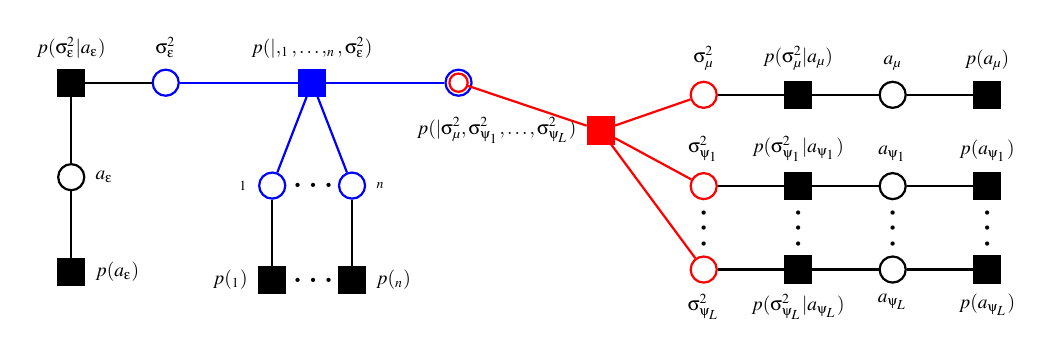
\begin{tikzpicture} [
		auto, node distance=1.2cm, every loop/.style={},
		thick,stochastic node/.style={circle,draw,font=\sffamily\Large\bfseries},
		factor/.style={regular polygon,regular polygon sides=4}
	]
	
	% Fragment for factor p(y | nu, zeta, sigsqeps):
	\node [
		fill = blue, factor, draw = blue, scale = 1,
		label = above:\scriptsize{$p ( \by | \bnu, \bzeta_1, \dots, \bzeta_n, \sigsqeps )$}
	] (py) {};
	\node [
		stochastic node, draw = blue, scale = 1,
		label = above:\scriptsize{$\bnu$}
	] (nu) [right = 1.5cm of py] {};
	\node [
		stochastic node, draw = blue, scale = 1,
		label = left:\scriptsize{$\bzeta_1$}
	] (zeta1) [below left = 1cm and 0.2cm of py] {};
	\node [
		stochastic node, draw = blue, scale=1,
		label = right:\scriptsize{$\bzeta_n$}
	] (zetaN) [below right = 1cm and 0.2cm of py] {};
	\node [font = \Large] (zeta_dots) at ($(zeta1)!0.54!(zetaN)$) {$\dots$};
	\node [
		stochastic node, draw = blue, scale=1,
		label = above:\scriptsize{$\sigsqeps$}
	] (sigsqeps) [left = 1.5cm of py] {};
	
	% Fragment for factor p(nu | sigsqmu, sigsqpsi1, ..., sigsqpsiL):
	\node [
		fill = red, factor, draw = red, scale = 1,
		label = left:\scriptsize{$p ( \bnu | \sigsqmu, \sigsqpsi{1}, \dots, \sigsqpsi{L} )$}
	] (pnu) [below right = 0.3cm and 1.5cm of nu] {};
	\node[stochastic node, draw = red, scale = 0.7] (nu_inner) at (nu.center) {};
	\node [
		stochastic node, draw = red, scale=1,
		label = above:\scriptsize{$\sigsqpsi{1}$}
	] (sigsqpsi1) [below right = 0.4cm and 1cm of pnu] {};
	\node [
		stochastic node, draw = red, scale=1,
		label = below:\scriptsize{$\sigsqpsi{L}$}
	] (sigsqpsiL) [below = 0.7cm of sigsqpsi1] {};
	\node [font = \Large, rotate=-90] (sigsqpsi_dots) at ($(sigsqpsi1)!0.53!(sigsqpsiL)$) {$\dots$};
	\node [
		stochastic node, draw = red, scale=1,
		label = above:\scriptsize{$\sigsqmu$}
	] (sigsqmu) [above = 0.8cm of sigsqpsi1] {};
	
	% Fragments for factors p(zeta1) ... p(zetaN):
	\node [
		fill, factor, draw, scale = 1,
		label = left:\scriptsize{$p ( \bzeta_1 )$}
	] (pzeta1) [below of =  zeta1] {};
	\node [
		fill, factor, draw, scale = 1,
		label = right:\scriptsize{$p ( \bzeta_n )$}
	] (pzetaN) [below of =  zetaN] {};
	\node [font = \Large] (pzeta_dots) at ($(pzeta1)!0.54!(pzetaN)$) {$\dots$};
	
	% Fragment for factor p(sigsqeps | aeps):
	\node [
		fill, factor, draw, scale = 1,
		label = above:\scriptsize{$p ( \sigsqeps | \aeps )$}
	] (psigsqeps) [left of = sigsqeps] {};
	\node [
		stochastic node, draw, scale=1,
		label = right:\scriptsize{$\aeps$}
	] (aeps) [below of = psigsqeps] {};
	
	% Fragment for factor p(aeps):
	\node [
		fill, factor, draw, scale = 1,
		label = right:\scriptsize{$p ( \aeps )$}
	] (paeps) [below of = aeps] {};
	
	% Fragment for factor p(sigsqmu | amu):
	\node [
		fill, factor, draw, scale = 1,
		label = above:\scriptsize{$p ( \sigsqmu | \amu )$}
	] (psigsqmu) [right of = sigsqmu] {};
	\node [
		stochastic node, draw, scale=1,
		label = above:\scriptsize{$\amu$}
	] (amu) [right of = psigsqmu] {};
	
	% Fragment for factor p(amu):
	\node [
		fill, factor, draw, scale = 1,
		label = above:\scriptsize{$p ( \amu )$}
	] (pamu) [right of = amu] {};
	
	% Fragments for factors p(sigsqpsi1 | apsi1) ... p(sigsqpsiL | apsiL):
	\node [
		fill, factor, draw, scale = 1,
		label = above:\scriptsize{$p ( \sigsqpsi{1} | \apsi{1} )$}
	] (psigsqpsi1) [right of = sigsqpsi1] {};
	\node [
		stochastic node, draw, scale = 1,
		label = above:\scriptsize{$ \apsi{1} $}
	] (apsi1) [right of = psigsqpsi1] {};
	\node [
		fill, factor, draw, scale = 1,
		label = below:\scriptsize{$p ( \sigsqpsi{L} | \apsi{L} )$}
	] (psigsqpsiL) [right of = sigsqpsiL] {};
	\node [
		stochastic node, draw, scale = 1,
		label = below:\scriptsize{$ \apsi{L} $}
	] (apsiL) [right of = psigsqpsiL] {};
	\node [font = \Large, rotate=-90] (psigsqpsi_dots) at ($(psigsqpsi1)!0.53!(psigsqpsiL)$) {$\dots$};
	\node [font = \Large, rotate=-90] (apsi_dots) at ($(apsi1)!0.53!(apsiL)$) {$\dots$};
	
	% Fragments for factors p(apsi1) ... p(apsiL):
	\node [
		fill, factor, draw, scale = 1,
		label = above:\scriptsize{$p ( \apsi{1} )$}
	] (papsi1) [right of = apsi1] {};
	\node [
		fill, factor, draw, scale = 1,
		label = below:\scriptsize{$p ( \apsi{L} )$}
	] (papsiL) [right of = apsiL] {};
	\node [font = \Large, rotate=-90] (papsi_dots) at ($(papsi1)!0.53!(papsiL)$) {$\dots$};
	
	% Construct edges:
	\path[every node/.style={font=\sffamily\small}]
	
	% Edges around fragment for factor p(y | nu, zeta1, ..., zetaN, sigsqeps):
	(py)
		edge [blue] node {} (nu)
		edge [blue] node {} (zeta1)
		edge [blue] node {} (zetaN)
		edge [blue] node {} (sigsqeps)
	
	% Edges around fragment for factor p(nu | sigsqmu, sigsqpsi1, ..., sigsqpsiL):
	(pnu)
		edge [red] node {} (nu_inner)
		edge [red] node {} (sigsqmu)
		edge [red] node {} (sigsqpsi1)
		edge [red] node {} (sigsqpsiL)
	
	% Edges around fragments for factors p(zeta1) ... p(zetaN):
	(pzeta1) edge node {} (zeta1)
	(pzetaN) edge node {} (zetaN)
	
	% Edges around fragment for factor p(sigsqeps | aeps):
	(psigsqeps)
		edge node {} (sigsqeps)
		edge node {} (aeps)
	
	% Edges around fragment for factor p(aeps):
	(paeps)
		edge node {} (aeps)
	
	% Edges around fragment for factor p(sigsqmu | amu):
	(psigsqmu)
		edge node {} (sigsqmu)
		edge node {} (amu)
	
	% Edges around fragment for factor p(amu):
	(pamu)
		edge node {} (amu)
	
	% Edges around fragments for factors p(sigsqpsi1 | apsi1) ... p(sigsqpsiL | apsiL):
	(psigsqpsi1)
		edge node {} (sigsqpsi1)
		edge node {} (apsi1)
	(psigsqpsiL)
		edge node {} (sigsqpsiL)
		edge node {} (apsiL)
	
	% Edges around fragments for factors p(apsi1) ... p(apsiL):
	(papsi1)
		edge node {} (apsi1)
	(papsiL)
		edge node {} (apsiL);
	
	\end{tikzpicture}
\caption{The factor graph for the Bayesian FPCA model in \eqref{bayes_fpca_mod}.}
\label{fig:fg_fpca}
\end{figure}

%% Exponential Family Form

\subsubsection{Exponential Family Form}
\label{sec:exp_fam_form}

A key step in deriving and implementing VMP algorithms is the representation of probability density functions
in exponential family form: $p (\bx) \propto \exp \{ \T{\bT(x)} \bdeta \}$, where $\bT (x)$ is a vector of sufficient
statistics that identify the distributional family, and $\bdeta$ is the natural parameter vector;
the messages in \eqref{nu_zeta_q_dens_funcs} are typically in the exponential family of density functions.
\citeA{wand17} explains how natural parameter vectors play a central role in the messages that are
passed within and between factor graph fragments. In particular, the natural parameter vectors for the
optimal $q$-density functions in \eqref{nu_zeta_q_dens_funcs} take the form

\begin{align}
\begin{split}
	\npq{\bnu} &=
		\np{p (\by | \bnu, \bzeta_1, \dots, \bzeta_n, \sigsqeps)}{\bnu} +
		\np{p (\bnu | \sigsqmu, \sigsqpsi{1}, \dots, \sigsqpsi{L})}{\bnu} \\
	\npq{\bzeta_i} &=
		\np{p (\by | \bnu, \bzeta_1, \dots, \bzeta_n, \sigsqeps)}{\bzeta_i} +
		\np{p (\bzeta_i)}{\bzeta_i} , \quad i = 1, \dots, n.
\end{split}
\label{etaq}
\end{align}

Before introducing the exponential family forms for key distributions in the VMP setting, we outline some
matrix and vector operators. We define the $\vect$ and $\vech$ operators,
which are well-established \cite<e.g.>{gentle07}.
For a $d_1 \times d_2$ matrix, the $\vect$ operator concatenates the columns of the matrix from left to right.
For a $d_1 \times d_1$ matrix, the $\vech$ operator concatenates the columns of the matrix after removing
the above diagonal elements. For example, suppose that $\bA = [\begin{array}{c c} \T{(2, -3)} & \T{(-1, 1)} \end{array}]$.
Then $\vect (\bA) = \T{(2, -3, -1, 1)}$ and $\vech (\bA) = \T{(2, -3, 1)}$.
For a $d^2 \times 1$ vector
$\ba$, $\vect^{-1} (\ba)$ is the $d \times d$ matrix such that $\vect \{\vect^{-1} (\ba)\} = \ba$. Additionally, the matrix
$\bD_d$ is the duplication matrix of order $d$, and it is such that $\bD_d \vech (\bA) = \vect (\bA)$ for a
$d \times d$ symmetric matrix $\bA$. Furthermore, $\bD_d^{+} \equiv (\T{\bD_d} \bD_d)^{-1} \T{\bD_d}$ is the
Moore-Penrose inverse of $\bD_d$, where $\bD_d^+ \vect (\bA) = \vech(\bA)$.

Now we describe the exponential family form for the normal distribution.
For a $d \times 1$ multivariate normal
random vector $\bx \sim \normal (\bmu, \bSigma)$, the probability density function of $\bx$ can be shown to satisfy

\begin{equation}
	p(\bx) = \exp \left\{ \T{\bT_{\vect} (\bx)} \bdeta_{\vect} - A_{\vect} (\bdeta_{\vect}) - \frac{d}{2} \log (2 \pi) \right\},
\label{vec_repn}
\end{equation}

\noindent where $\bT_{\vect} (\bx) \equiv \T{\{ \T{\bx}, \T{\vect ( \bx \T{\bx} )} \}}$ is the vector of sufficient statistics
and $\bdeta_{\vect} \equiv \T{( \T{\bdeta_{\vect, 1}}, \T{\bdeta_{\vect, 2}} )} \equiv \T{[ \T{( \bSigma^{-1} \bmu )},
-\frac12 \T{\{ \vect (\bSigma^{-1}) \}} ]}$ is the natural parameter vector.
The function $A_{\vect} (\bdeta_{\vect}) =
-\frac14 \T{\bdeta}_{\vect, 1} \{ \vect^{-1} (\bdeta_{\vect, 2}) \}^{-1} \bdeta_{\vect, 1}
- \frac12 \log | -2 \vect^{-1} (\bdeta_{\vect, 2}) |$ is the log-partition function.
The inverse mapping of the natural parameter vector is \cite[equation~S.4]{wand17}

\begin{equation}
	\bmu = -\frac12 \left\{ \vect^{-1} (\bdeta_{\vect, 2}) \right\}^{-1} \bdeta_{\vect, 1} \quad
	\text{and} \quad
	\bSigma = -\frac12 \left\{ \vect^{-1} (\bdeta_{\vect, 2}) \right\}^{-1}.
\label{gauss_vec_comm_params}
\end{equation}

\noindent We will refer to the representation of the multivariate normal probability density function in
\eqref{vec_repn} as the \emph{vec-based representation}.

Alternatively, a more storage-economical
representation of the multivariate normal probability density function is the \emph{vech-based representation}:

\[
	p (\bx) = \exp \left\{ \T{\bT_{\vech} (\bx)} \bdeta_{\vech} - A_{\vech} (\bdeta_{\vech}) - \frac{d}{2} \log (2 \pi) \right\},
\]

\noindent where the vector of sufficient statistics, the natural parameter vector and the log-partition function are,
$\bT_{\vech} (\bx) \equiv \T{\{ \T{\bx}, \T{\vect ( \bx \T{\bx} )} \}}$,
$\bdeta_{\vech} \equiv \T{( \T{\bdeta_{\vech, 1}}, \T{\bdeta_{\vech, 2}} )} \equiv \T{[ \T{( \bSigma^{-1} \bmu )},
-\frac12 \T{ \T{\bD_d} \{ \vect (\bSigma^{-1}) \}} ]}$ and
$A_{\vech} (\bdeta_{\vech}) = -\frac14 \T{\bdeta}_{\vech, 1} \{ \vect^{-1} (\bD_d^{+ \intercal} \bdeta_{\vech, 2}) \}^{-1}
\bdeta_{\vech, 1} - \frac12 \log | -2 \vect^{-1} (\bD_d^{+ \intercal} \bdeta_{\vech, 2}) |$, respectively.
The inverse mapping of the natural parameter vector under the vech-based representation is

\begin{equation}
	\bmu = -\frac12 \left\{ \vect^{-1} (\bD_d^{+ \intercal}\bdeta_{\vech, 2}) \right\}^{-1} \bdeta_{\vech, 1} \quad
	\text{and} \quad
	\bSigma = -\frac12 \left\{ \vect^{-1} (\bD_d^{+ \intercal}\bdeta_{\vech, 2}) \right\}^{-1}.
\label{gauss_vech_comm_params}
\end{equation}

The other major distribution within the exponential family that is pivotal for this article is the inverse-$\chi^2$ distribution.
A random variable $x$ has an inverse-$\chi^2$ distribution with shape parameter $\xi > 0$ and scale parameter
$\lambda > 0$ if the probability density function of $x$ is

\[
	p(x) = 
		\frac{(\lambda/2)^{\xi/2}}{\Gamma (\xi/2)}
		x^{-(\xi + 2)/2} \exp \left( -\frac{\lambda}{2 x} \right) \ind (x > 0),
\]

\noindent where the vector of sufficient statistics, the natural parameter vector and the log-partition function are
$\bT (x) \equiv \T{( \log (x), 1/x )}$, $\bdeta = \T{(\eta_1, \eta_2)} = \T{\{-\frac12 (\xi + 2), -\frac{\lambda}{2} \}}$
and $A(\bdeta) \equiv \log \{ \Gamma (\xi/2) \} - \frac{\xi}{2} \log (\lambda/2)$, respectively. Note that
$\Gamma (z) \equiv \int_0^\infty u^{z - 1} e^u du$ is the gamma function,
$\ind (\cdot)$ is the indicator function, $\zeta > 0$ is the scale parameter and $\lambda > 0$ is the shape parameter.
The inverse mapping of the natural parameter vector is
$\xi = -2 \eta_1 - 2$ and $\lambda = -2 \eta_2$.

We introduce two new fragments that are required for variational inference via VMP for the FPCA model. These
are the \emph{functional principal component Gaussian likelihood fragment} (blue in Figure \ref{fig:fg_fpca})
and the \emph{functional principal component Gaussian penalization fragment} (red in Figure \ref{fig:fg_fpca}).
The fragments for $p (\bzeta_1), \dots, p (\zeta_n)$ are \emph{Gaussian prior fragments}
\cite[Section~4.1.1]{wand17}; the fragments for $p (\sigsqeps | \aeps)$, $p (\sigsqmu | \amu)$ and
$p (\sigsqpsi{1} | \apsi{1}), \dots, p (\sigsqpsi{L} | \apsi{L})$ are univariate versions of the \emph{iterated inverse
G-Wishart fragment} \cite[Algorithm~2]{maestrini20}; and $p (\aeps)$, $p (\amu)$ and $p (\apsi{1}), \dots, p (\apsi{L})$
are univariate versions of the \emph{inverse G-Wishart prior fragment} \cite[Algorithm~1]{maestrini20}.

%%%%%%%%%%%%%% Functional Principal Component Gaussian Likelihood Fragment

\subsection{Functional Principal Component Gaussian Likelihood Fragment}
\label{sec:fpca_gauss_lik_frag}

The message from $p (\by | \bnu, \bzeta_1, \dots, \bzeta_n, \sigsqeps)$ to $\bnu$ can be shown to be
proportional to a multivariate normal density function, with natural parameter vector

\begin{equation}
	\np{p (\by | \bnu, \bzeta_1, \dots, \bzeta_n, \sigsqeps)}{\bnu}
		\longleftarrow
			\begin{bmatrix}
				\E_q (1/\sigsqeps) \displaystyle\sum_{i=1}^n \T{\left\{
					\T{\E_q (\bzetatilde_i)} \otimes \bC_i
				\right\}} \by_i \\
				-\frac12 \E_q (1/\sigsqeps) \displaystyle\sum_{i=1}^n \vect \left\{
					\E_q (\bzetatilde_i \T{\bzetatilde_i}) \otimes (\T{\bC_i} \bC_i)
				\right\}
			\end{bmatrix},
\label{np_lik_nu}
\end{equation}

\noindent where $\bzetatilde_i \equiv \T{(1, \T{\bzeta_i})}, \quad i = 1, \dots, n$. Note that the natural
parameter vector in \eqref{np_lik_nu} is within the vec-based representation of a normal probability density function.
In preliminary simulations, we found that computations using the vech-based representation were enormously hindered
by the need to use a huge Moore-Penrose inverse matrix. For instance, consider the case where
there are two basis functions ($L = 2$) and 25 O'Sullivan penalized spline basis functions ($K = 25$) for nonparametric
regression. In this instance, the vector $\bnu$ is $81 \times 1$ ($d = 81$) and the Moore-Penrose inverse matrix
$\bD_{81}^+$ has dimension $3321 \times 6561$, inhibiting the computational speed. For this reason, we have
decided to use the vec-based representation for $\msg{p (\by | \bnu, \bzeta_1, \dots, \bzeta_n, \sigsqeps)}{\bnu}$,
which does not require the
use of a Moore-Penrose inverse matrix.

For each $i = 1, \dots, n$, the message from $p (\by | \bnu, \bzeta_1, \dots, \bzeta_n, \sigsqeps)$ to $\bzeta_i$
is proportional to a multivariate normal density function, with natural parameter vector

\begin{equation}
	\np{p (\by | \bnu, \bzeta_1, \dots, \bzeta_n, \sigsqeps)}{\bzeta_i}
		\longleftarrow
			\begin{bmatrix}
				\E_q (1/\sigsqeps) \left\{
					\T{\E_q (\Vpsi)} \T{\bC_i} \by_i - \E_q (\hmupsi{i})
				\right\} \\
				-\frac12 \E_q (1/\sigsqeps) \T{\bD_L} \vect \{ \E_q (\Hpsi{i}) \}
			\end{bmatrix},
\label{np_lik_zeta}
\end{equation}

\noindent where $ \Vpsi \equiv [\begin{array}{ccc} \nupsi{1} & \dots & \nupsi{L} \end{array}]$,
$\hmupsi{i} \equiv \T{\Vpsi} \T{\bC_i} \bC_i \numu$ and $\Hpsi{i} \equiv \T{\Vpsi} \T{\bC_i} \bC_i \Vpsi$.
Note that this natural parameter vector is within the vech-based representation of a normal probability density function.

The message from $p (\by | \bnu, \bzeta_1, \dots, \bzeta_n, \sigsqeps)$ to $\sigsqeps$
is an inverse-$\chi^2$ density function, with natural parameter vector

\begin{equation}
	\np{p (\by | \bnu, \bzeta_1, \dots, \bzeta_n, \sigsqeps)}{\sigsqeps}
		\longleftarrow
			\begin{bmatrix}
				-\frac12 \displaystyle\sum_{i=1}^n T_i \\
				-\frac12 \displaystyle\sum_{i=1}^n \E_q \left\{ \T{\left(
					\by_i - \bC_i \bV \bzetatilde_i
				\right)} \left(
					\by_i - \bC_i \bV \bzetatilde_i
				\right) \right\}
			\end{bmatrix},
\label{np_lik_sigsqeps}
\end{equation}

\noindent where $\bV \equiv [\begin{array}{cccc} \numu & \nupsi{1} & \dots & \nupsi{L} \end{array}]$.
Note that the inverse-$\chi^2$ density function message that is passed
to $\sigsqeps$ is part of the inverse G-Wishart class of density functions. In keeping
with the formalisms set out in \citeA{maestrini20},
a graph message is also required for conjugate variational inference.
According to Section 7.4 of \citeA{maestrini20},
the auxiliary-based hierarchical prior specification of $\sigsqeps$ in \eqref{bayes_fpca_mod} requires a
graphical message of the form

\begin{equation}
	G_{p (\by | \bnu, \bzeta_1, \dots, \bzeta_n, \sigsqeps) \rightarrow \sigsqeps}
		\longleftarrow
			G_{\text{full}}.
\label{G_lik_sigsqeps}
\end{equation}

\noindent See \citeA{maestrini20} for further details on graphical parameters in inverse G-Wishart and\
inverse-$\chi^2$ density functions.

Pseudocode for the functional principal component
Gaussian likelihood fragment is presented in Algorithm \ref{alg:fpca_gauss_lik_frag}.
A derivation of all the relevant expectations and natural parameter vector updates is provided in Appendix
\ref{app:fpca_gauss_lik_frag}.

\begin{algorithm}
	\caption{
		Pseudocode for the functional principal component Gaussian likelihood fragment.
	}
	\label{alg:fpca_gauss_lik_frag}
	\begin{algorithmic}[1]
		\Inputs
			\begin{varwidth}[t]{\linewidth} $
				\np{\bnu}{p (\by | \bnu, \bzeta_1, \dots, \bzeta_n, \sigsqeps)}, \quad
				\{ \np{\bzeta_i}{p (\by | \bnu, \bzeta_1, \dots, \bzeta_n, \sigsqeps)} : i = 1, \dots, n \}
			$\par$
				\{
					\np{\sigsqeps}{p (\by | \bnu, \bzeta_1, \dots, \bzeta_n, \sigsqeps)}, \
					G_{\sigsqeps \rightarrow p (\by | \bnu, \bzeta_1, \dots, \bzeta_n, \sigsqeps)}
				\}
			$ \end{varwidth}
		\Updates
			\State Update posterior expectations.
				\Comment{see Appendix \ref{app:fpca_gauss_lik_frag}}
			\State Update $\np{p (\by | \bnu, \bzeta_1, \dots, \bzeta_n, \sigsqeps)}{\bnu}$
				\Comment{equation \eqref{np_lik_nu}}
			\For{$i = 1, \dots, n$}
				\State Update $\np{p (\by | \bnu, \bzeta_1, \dots, \bzeta_n, \sigsqeps)}{\bzeta_i}$
					\Comment{equation \eqref{np_lik_zeta}}
			\EndFor
			\State Update $\np{p (\by | \bnu, \bzeta_1, \dots, \bzeta_n, \sigsqeps)}{\sigsqeps}$
				\Comment{equation \eqref{np_lik_sigsqeps}}
			\State Update $G_{p (\by | \bnu, \bzeta_1, \dots, \bzeta_n, \sigsqeps) \rightarrow \sigsqeps}$
				\Comment{equation \eqref{G_lik_sigsqeps}}
		\Outputs
			\begin{varwidth}[t]{\linewidth} $
				\np{p (\by | \bnu, \bzeta_1, \dots, \bzeta_n, \sigsqeps)}{\bnu}, \quad
				\{ \np{p (\by | \bnu, \bzeta_1, \dots, \bzeta_n, \sigsqeps)}{\bzeta_i} : i = 1, \dots, n \}
			$\par$
				\{
					\np{p (\by | \bnu, \bzeta_1, \dots, \bzeta_n, \sigsqeps)}{\sigsqeps}, \
					G_{p (\by | \bnu, \bzeta_1, \dots, \bzeta_n, \sigsqeps) \rightarrow \sigsqeps}
				\}
			$ \end{varwidth}
	\end{algorithmic}
\end{algorithm}

%%%%%%%%%%%%%% Mean and FPC Gaussian Penalization Fragment

\subsection{Functional Principal Component Gaussian Penalization Fragment}
\label{sec:mean_fpc_gauss_pen_frag}

The message passed from $p (\bnu | \sigsqmu, \sigsqpsi{1}, \dots, \sigsqpsi{L})$ to $\bnu$ can be shown to
be a multivariate normal density function, with natural parameter vector

\begin{equation}
	\np{p (\bnu | \sigsqmu, \sigsqpsi{1}, \dots, \sigsqpsi{L})}{\bnu}
		\longleftarrow
			\begin{bmatrix}
				\E_q (\Sigmanu^{-1}) \munu \\
				-\frac12 \vect \left\{ \E_q (\Sigmanu^{-1}) \right\}
			\end{bmatrix}.
\label{np_pen_nu}
\end{equation}

\noindent where $\munu \equiv \T{(\T{\mumu}, \T{\mupsi{1}}, \dots, \T{\mupsi{L}})}$ and
$\Sigmanu \equiv \blockdiag (\bSigma_\mu, \bSigma_{\psi_1}, \dots, \bSigma_{\psi_L})$.
The natural parameter vector in \eqref{np_pen_nu} is within the
vec-based representation of the message to $\bnu$, as opposed to
a storage-economical vech-based representation, for the same reasons that are outlined in the discussion
following \eqref{np_lik_nu}.

The message from $p (\bnu | \sigsqmu, \sigsqpsi{1}, \dots, \sigsqpsi{L})$ to $\sigsqmu$ is an inverse-$\chi^2$
density function, with natural parameter vector

\begin{equation}
	\np{p (\bnu | \sigsqmu, \sigsqpsi{1}, \dots, \sigsqpsi{L})}{\sigsqmu}
		\longleftarrow
			\begin{bmatrix}
				-\frac{K}{2} \\
				-\frac12 \E_q (\T{\umu} \umu)
			\end{bmatrix}.
\label{np_pen_sigsqmu}
\end{equation}

Similarly, the message passed from $p (\bnu | \sigsqmu, \sigsqpsi{1}, \dots, \sigsqpsi{L})$ to $\sigsqpsi{l}$,
$l = 1, \dots, L$, is an inverse-$\chi^2$ density function, with natural parameter vector

\begin{equation}
	\np{p (\bnu | \sigsqmu, \sigsqpsi{1}, \dots, \sigsqpsi{L})}{\sigsqpsi{l}}
		\longleftarrow
			\begin{bmatrix}
				-\frac{K}{2} \\
				-\frac12 \E_q (\T{\upsi{l}} \upsi{l})
			\end{bmatrix}.
\label{np_pen_sigsqpsi}
\end{equation}

Finally, recall the discussion following \eqref{np_lik_sigsqeps}.
Each of the messages to the variance parameters $\sigsqmu,
\sigsqpsi{1}, \dots, \sigsqpsi{L}$ must be paired with a graph message. For the same reasons that were used to
justify the graphical message in \eqref{G_lik_sigsqeps}, the graph messages received by $\sigsqmu,
\sigsqpsi{1}, \dots, \sigsqpsi{L}$ are, respectively,

\begin{equation}
	G_{p (\bnu | \sigsqmu, \sigsqpsi{1}, \dots, \sigsqpsi{L}) \rightarrow \sigsqmu}
		\longleftarrow
			G_{\text{full}} \quad
	\text{and} \quad
	G_{p (\bnu | \sigsqmu, \sigsqpsi{1}, \dots, \sigsqpsi{L}) \rightarrow \sigsqpsi{l}}
		\longleftarrow
			G_{\text{full}}, \quad l = 1, \dots, L.
\label{G_pen}
\end{equation}

Pseudocode for the functional principal component Gaussian penalization fragment is presented in Algorithm
\ref{alg:mean_fpc_gauss_pen_frag}.
A derivation of all the relevant expectations and natural parameter vector updates is provided in Appendix
\ref{app:mean_fpc_gauss_pen_frag}.

\begin{algorithm}
	\caption{
		Pseudocode for the functional principal component Gaussian penalization fragment.
	}
	\label{alg:mean_fpc_gauss_pen_frag}
	\begin{algorithmic}[1]
		\Inputs
			\begin{varwidth}[t]{\linewidth} $
				\np{\bnu}{p (\bnu | \sigsqmu, \sigsqpsi{1}, \dots, \sigsqpsi{L})}, \quad
				\{
					\np{\sigsqmu}{p (\bnu | \sigsqmu, \sigsqpsi{1}, \dots, \sigsqpsi{L})}, \
					G_{\sigsqmu \rightarrow p (\bnu | \sigsqmu, \sigsqpsi{1}, \dots, \sigsqpsi{L})}
				\}
			$\par$
				\{
					\np{\sigsqpsi{l}}{p (\bnu | \sigsqmu, \sigsqpsi{1}, \dots, \sigsqpsi{L})}, \
					G_{\sigsqpsi{l} \rightarrow p (\bnu | \sigsqmu, \sigsqpsi{1}, \dots, \sigsqpsi{L})} :
					l = 1, \dots, L
				\}
			$ \end{varwidth}
		\Updates
			\State Update posterior expectations.
				\Comment{see Appendix \ref{app:mean_fpc_gauss_pen_frag}}
			\State Update $\np{p (\bnu | \sigsqmu, \sigsqpsi{1}, \dots, \sigsqpsi{L})}{\bnu}$
				\Comment{equation \eqref{np_pen_nu}}
			\State Update $\np{p (\bnu | \sigsqmu, \sigsqpsi{1}, \dots, \sigsqpsi{L})}{\sigsqmu}$
				\Comment{equation \eqref{np_pen_sigsqmu}}
			\State Update $G_{p (\bnu | \sigsqmu, \sigsqpsi{1}, \dots, \sigsqpsi{L}) \rightarrow \sigsqmu}$
				\Comment{equation \eqref{G_pen}}
			\For{$l = 1, \dots, L$}
				\State Update $\np{p (\bnu | \sigsqmu, \sigsqpsi{1}, \dots, \sigsqpsi{L})}{\sigsqpsi{l}}$
					\Comment{equation \eqref{np_pen_sigsqpsi}}
				\State Update $G_{p (\bnu | \sigsqmu, \sigsqpsi{1}, \dots, \sigsqpsi{L}) \rightarrow \sigsqpsi{l}}$
					\Comment{equation \eqref{G_pen}}
			\EndFor
		\Outputs
			\begin{varwidth}[t]{\linewidth} $
				\np{p (\bnu | \sigsqmu, \sigsqpsi{1}, \dots, \sigsqpsi{L})}{\bnu}, \quad
				\{
					\np{p (\bnu | \sigsqmu, \sigsqpsi{1}, \dots, \sigsqpsi{L})}{\sigsqmu}, \
					G_{p (\bnu | \sigsqmu, \sigsqpsi{1}, \dots, \sigsqpsi{L}) \rightarrow \sigsqmu}
				\}
			$\par$
				\{
					\np{p (\bnu | \sigsqmu, \sigsqpsi{1}, \dots, \sigsqpsi{L})}{\sigsqpsi{l}}, \
					G_{p (\bnu | \sigsqmu, \sigsqpsi{1}, \dots, \sigsqpsi{L}) \rightarrow \sigsqpsi{l}} :
					l = 1, \dots, L
				\}
			$ \end{varwidth}
	\end{algorithmic}
\end{algorithm}

%%%%%%%%%%% POST-VMP  STEPS  %%%%%%%%%%%

\section{Post-VMP Steps}
\label{sec:post_vmp_steps}

The FPCA model for curve estimation \eqref{yhat}, which has its genesis in the Karhunen-Lo\`{e}ve decomposition
\eqref{kl_expansion}, relies on orthogonal functional principal component
eigenfunctions and independent vectors of scores with uncorrelated entries.
However, the variational Bayesian FPCA resulting from a VMP treatment
does not enforce any orthogonality restrictions on the resulting eigenfunctions. Although curve estimation is still
valid without these constraints, interpretation of the analysis is more straightforward with orthogonal
eigenfunctions. Furthermore, the eigenfunctions are not guaranteed to be normalized.
In the following sections, we outline
a sequence of post-VMP steps that aid inference and interpretability for variational Bayes-based FPCA.

%%%%%%%%%%%%%% Establishing the Optimal Posterior Density Functions

\subsection{Establishing the Optimal Posterior Density Functions}
\label{sec:opt_dens_funcs}

We are primarily concerned with the optimal posterior density functions for the vector of spline coefficients for
the mean function and eigenfunctions $\bnu$ and the vectors of principal component scores $\bzeta_1, \dots,
\bzeta_n$. Upon convergence of the VMP algorithm, the natural parameter vectors for these optimal posterior density
functions can be computed via \eqref{etaq}.
The optimal posterior density for each of these parameters is a Gaussian density
function, where the mean vector $\E_q (\bnu)$ and covariance matrix $\Cov_q (\bnu)$ for $q^* (\bnu)$
can be computed from
\eqref{gauss_vec_comm_params}, and the corresponding parameters $\E_q (\bzeta_i)$ and $\Cov_q (\bzeta_i)$
for $q^* (\bzeta_i)$, $i = 1, \dots, n$, can be
computed from \eqref{gauss_vech_comm_params}. Note that we partition $\E_q (\bnu)$ as $\E_q (\bnu) =
\T{\{ \T{\E_q (\numu)}, \T{\E_q (\nupsi{1})}, \dots, \T{\E_q (\nupsi{L})} \}}$.

%%%%%%%%%%%%%% Establishing Multivariate Version of the Karhunen-Lo\`{e}ve Decomposition

\subsection{Establishing the Karhunen-Lo\`{e}ve Decomposition}
\label{sec:biorthogonal}

In this section, we outline a sequence of steps to establish orthogonal
functional principal component eigenfunctions and uncorrelated scores.
Note that we will treat the estimated functional principal component eigenfunctions as fixed curves that
are estimated from the posterior mean of the spline coefficients $\E_q (\bnu)$. As a consequence, the pointwise
posterior variance in the response curve estimates result from the variance in the principal component scores
alone. This treatment is in line with standard approaches to FPCA, where the randomness in the model is
generated by the scores  \cite<e.g.>{yao05, benko09}.

Now, we outline the steps to construct orthogonal functional principal component eigenfunctions and
uncorrelated scores. The existence and uniqueness of the eigenfunctions are justified by Theorem \ref{thm:orth_basis}.
First, set up an equidistant grid of design points $\bt_g = \T{(t_{g1}, \dots, t_{gn_g})}$,
where $t_{g1} = 0$, $t_{gn_g} = 1$ and $n_g$ is the length of the grid. Then define $\bC_g$ in an analogous fashion
to \eqref{C_mat}: $\bC_g \equiv [ \begin{array}{ccccc} \bone_{n_g} & \bt_g & z_1 (\bt_g) & \cdots & z_K (\bt_g)
\end{array}]$, where $\bone_{n_g}$ is an $n_g \times 1$ vector of ones.
Establish the posterior estimates of the mean function $\E_q \{ \mu (\bt_g) \} = \bC_g \E_q (\numu)$
and the functional principal components eigenfunctions $\E_q \{ \psi_l (\bt_g) \} = \bC_g \E_q (\nupsi{l})$,
$l = 1, \dots, L$. Then define the matrix $\bPsi$ such that
$\bPsi \equiv [\begin{array}{ccc} \E_q \{ \psi_1 (t_g) \} & \cdots & \E_q \{ \psi_L (t_g) \} \end{array}]$.
Establish the singular value decomposition of $\bPsi$ such that $\bPsi = \bU_\psi \bD_\psi \T{\bV}_\psi$,
where $\bU_\psi$ is an $n_g \times L$ matrix consisting of the first $L$ left singular vectors of $\bPsi$,
$\bV_\psi$ is an $L \times L$ matrix consisting of the right singular vectors of $\bPsi$, and
$\bD_\psi$ is an $L \times L$ diagonal matrix consisting of the singular values of $\bPsi$.

Next, define $\bXi \equiv \T{[\begin{array}{ccc} \E_q (\bzeta_1) & \cdots & \E_q (\bzeta_n) \end{array}]}$.
Set $\bm_\zeta$ to be the $L \times 1$ sample mean vector of the column vectors of
$\bD_\psi \T{\bV}_\psi \T{\bXi}$, and set

\begin{equation}
	\muhat (\bt_g) \equiv \E_q \{ \mu (\bt_g) \} + \bU_\psi \bm_\zeta.
\label{mu_shift}
\end{equation}

\noindent Then set $\bC_\zeta$ to be the $L \times L$ sample covariance matrix of the
column vectors of $\bD_\psi \T{\bV}_\psi \T{\bXi} - \bm_\zeta \T{\bone_n}$ and establish its spectral decomposition
$\bC_\zeta = \bQ \bLambda \T{\bQ}$, where
$\bLambda$ is a diagonal matrix consisting of the eigenvalues of $\bC_\zeta$ in descending order along its
main diagonal and $\bQ$ is the orthogonal matrix consisting of the corresponding eigenvectors of $\bC_\zeta$ along
its columns.

Finally, define the matrices

\begin{equation}
	\bPsitilde \equiv \bU_\psi \bQ \bLambda^{1/2} \quad
	\text{and} \quad
	\bXitilde \equiv (\bXi \bV_\psi \bD_\psi - \bone_n \T{\bm_\zeta}) \bQ \bLambda^{-1/2}.
\label{psi_zeta_orth}
\end{equation}

\noindent Notice that $\bPsitilde$ is an $n_g \times L$ matrix and $\bXitilde$ is an $n \times L$ matrix. Next, partition
these matrices such that the $l$th column of $\bPsitilde$ is $\bpsitilde_l (\bt_g)$ and the $i$th row of $\bXitilde$ is
$(\zetatilde_{11}, \dots, \zetatilde_{1L})$.
The columns of $\bPsitilde$ are orthonormal vectors, but we require continuous curves that are orthonormal in
$L^2 [0, 1]$. We can adjust this by finding an approximation of $|| \bpsitilde_l ||$, $l = 1, \dots, L$, through numerical
integration. This allows us to establish estimates of the orthonormal functions $\psi^*_1, \dots, \psi^*_L$ in
\eqref{yhat} over the vector $\bt_g$ with

\begin{equation}
	\psihat_l (\bt_g) \equiv \frac{\bpsitilde_l (\bt_g)}{|| \bpsitilde_l ||}, \quad l = 1, \dots, L,
\label{psi_star}
\end{equation}

\noindent as well as estimates of the scores with
$\zetahat_{il} \equiv || \bpsitilde_l || \zetatilde_{il}$.
Lemma \ref{lem:response_est} outlines the construction of posterior curve estimation for the
response vectors $y_1 (\bt_g),
\dots, y_n (\bt_g)$. Proposition \ref{prop:bi_orthogonal} shows that the form of the predicted response vectors
in Lemma \ref{lem:response_est} is a vector version of the Karhunen-Lo\`{e}ve decomposition. Here, we define
$\bzetahat_i \equiv \T{(\zetahat_{i1}, \dots, \zetahat_{iL})}$, $i = 1, \dots, n$.

\begin{lemma}
	
	The posterior estimate for the response vector $y_i (\bt_g)$ is given by
	
	\begin{equation}
		\yhat_i (\bt_g) = \muhat (\bt_g) + \sum_{l=1}^L \zetahat_{il} \psihat_l (\bt_g), \quad i = 1, \dots, n.
	\label{post_curve_est}
	\end{equation}
	
\label{lem:response_est}
\end{lemma}

\begin{remark}
	
	The posterior estimates $\yhat_1 (\bt_g), \dots, \yhat_n (\bt_g)$ in \eqref{post_curve_est} are
	the same as those prior to the post-processing steps outlined above. That is,
	$\yhat_i (\bt_g) = \bC_g \E_q (\numu) + \sum_{l=1}^L \E_q (\zeta_{il}) \bC_g \E_q (\nupsi{l}),$
	where $\E_q (\numu)$ is the posterior estimate of $\numu$ from the VMP algorithm and similarly for
	$\E_q (\zeta_{il})$ and $\E_q (\nupsi{l})$. In summary, the post processing steps simply realign the mean function,
	orthogonalize and normalize the eigenfunctions and uncorrelate the scores, but do not affect the fits to the
	observed data.
	
\end{remark}

\begin{proposition}
	
	The vectors $\bzetahat_1, \dots, \bzetahat_N$ are independent and satisfy $\frac{1}{n} \sum_{i=1}^n \bzetahat_i =
	\bzero$ and $\frac{1}{n-1} \sum_{i=1}^n \bzetahat_i \bzetahat^{\intercal}_i = \diag (
	|| \psitilde_1 ||^2, \dots, || \psitilde_L ||^2)$.
	Furthermore, the vectors $\psihat_1 (\bt_g), \dots, \psihat_L (\bt_g)$ are eigenvectors of the sample
	covariance matrix of $\yhat_1 (\bt_g), \dots, \yhat_n (\bt_g)$.
	
\label{prop:bi_orthogonal}
\end{proposition}

\begin{remark}
	
	Proposition \ref{prop:bi_orthogonal} shows that the sample properties of the posterior estimates for the scores
	obey the assumptions of the scores in the Karhunen-Lo\`{e}ve decomposition in \eqref{kl_expansion}.
	Furthermore, the vectors $\psihat_1 (\bt_g), \dots, \psihat_L (\bt_g)$ respect the orthogonality conditions in $\ell^2$.
	Therefore, \eqref{post_curve_est} may be interpreted as a vector version of the truncated
	Karhunen-Lo\`{e}ve decomposition. As a consequence, the numerical estimates of
	$|| \psitilde_l ||^2$, $l = 1, \dots, L$ are the posterior estimates of the eigenvalues of the covariance operator
	$\Sigma$ (see the first paragraph of Section \ref{sec:fpca}).
	
\end{remark}

\noindent The proof of Lemma \ref{lem:response_est} is presented in Appendix \ref{app:proof_lem_response_est},
and the proof of Proposition \ref{prop:bi_orthogonal} is presented in Appendix \ref{app:proof_prop_bi_eigenfunctions}.

%%%%%%%%%%%  SIMULATIONS  %%%%%%%%%%%

\section{Simulations}
\label{sec:sims}

We illustrate the use of Algorithms \ref{alg:fpca_gauss_lik_frag} and \ref{alg:mean_fpc_gauss_pen_frag}
through a series of simulations of model \eqref{bayes_fpca_mod}. Pseudocode for the VMP algorithm is
provided in Algorithm \ref{alg:vmp_alg}.

\begin{algorithm}
	\caption{
		Generic VMP algorithm for the Gaussian response FPCA model \eqref{bayes_fpca_mod} with
		mean field restriction \eqref{fpca_mf_restrn}.
	}
	\label{alg:vmp_alg}
	\begin{algorithmic}[1]
		\Inputs All hyperparameters and observed data
		\Initialize All factor to stochastic node messages.
			\Comment{\citeA[Section 2.5]{wand17}}
		\Updates
			\While{$\lpyq$ has not converged}
				\State Update all stochastic node to factor messages.
					\Comment{\citeA[Section 2.5]{wand17}}
				\State Update the fragment for $p (\by | \bnu, \bzeta_1, \dots, \bzeta_n, \sigsqeps)$
					\Comment{Algorithm \ref{alg:fpca_gauss_lik_frag}}
				\State Update the fragment for $p (\sigsqeps | \aeps)$
					\Comment{\citeA[Algorithm 2]{maestrini20}}
				\State Update the fragment for $p (\aeps)$
					\Comment{\citeA[Algorithm 1]{maestrini20}}
				\State Update the fragment for $p (\bnu | \sigsqmu, \sigsqpsi{1}, \dots, \sigsqpsi{L})$
					\Comment{Algorithm \ref{alg:mean_fpc_gauss_pen_frag}}
				\For{$i = 1, \dots, n$}
					\State Update the fragment for $p (\bzeta_i)$
						\Comment{\citeA[Section 4.1.1]{wand17}}
				\EndFor
				\State Update the fragment for $p (\sigsqmu | \amu)$
					\Comment{\citeA[Algorithm 2]{maestrini20}}
				\State Update the fragment for $p (\amu)$
					\Comment{\citeA[Algorithm 1]{maestrini20}}
				\For{$i = 1, \dots, n$}
					\State Update the fragment for $p (\sigsqpsi{l} | \apsi{l})$
						\Comment{\citeA[Algorithm 2]{maestrini20}}
					\State Update the fragment for $p (\apsi{l})$
						\Comment{\citeA[Algorithm 1]{maestrini20}}
				\EndFor
			\EndWhile
			\State Rotate, translate and re-scale $\bPsi$ and $\bXi$.
				\Comment{Section \ref{sec:biorthogonal}}
		\Outputs $\muhat (\bt_g)$, $\psihat_1 (\bt_g), \dots, \psihat_L (\bt_g)$ and $\bzetahat_1, \dots, \bzetahat_n$.
	\end{algorithmic}
\end{algorithm}

\begin{figure}
	\centering
	\begin{subfigure}[t]{0.49\textwidth}
		\centering
		\includegraphics[width=2.9in]{images/response_curves.pdf}
	\caption{}
	\label{subfig:gauss_response_curves}
	\end{subfigure}
	%
	\begin{subfigure}[t]{0.49\textwidth}
		\centering
		\includegraphics[width=2.9in]{images/scores.pdf}
	\caption{}
	\label{subfig:gauss_response_scores}
	\end{subfigure}
	%
\caption{
	The results from one simulation of the Gaussian response FPCA model in \eqref{bayes_fpca_mod}. The
	simulation parameters are outlined in Section \ref{sec:sims}.
	In \subref{subfig:gauss_response_curves}, the simulated data are shown in black, while the VMP-based
	variational Bayes posterior estimates are presented in red and the corresponding MCMC estimates
	are shown in blue. In each panel, the solid lines represent
	the posterior mean, while the dashed line represents the 95\% pointwise credible sets for the mean.
	In \subref{subfig:gauss_response_scores}, we present the vector of scores for each of the
	randomly selected response curves,
	shown in black, as well as the VMP-based variational Bayes posterior estimates, shown in red, and the
	MCMC-based posterior estimates, shown in blue. The red and blue dots represent the VMP-based
	variational Bayes posterior means and the MCMC-based posterior means, respectively.
	The ellipses represent the 95\% credible contours.
}
\label{fig:gauss_resp_sim}
\end{figure}

%%%%%%%%%%%%%% Accuracy Assessment

\subsection{Accuracy Assessment}
\label{sec:acc_ass}

For model \eqref{bayes_fpca_mod}, we simulated 50 response curves with the number
of observations $T_i$ for the $i$th curve sampled uniformly over $\{ 20, 21, \dots, 30 \}$. Furthermore, the time
observations within the $i$th curve $\{ t_{i1}, \dots, t_{i T_i} \}$ were sampled uniformly over the interval $(0, 1)$,
while the residual variance $\sigsqeps$ was set to 1. The mean function was $\mu (t) = 3 \sin (\pi t)$
and the eigenfunctions were $\psi_1 (t) = \sqrt{2} \sin (2 \pi t)$ and $\psi_2 (t) = \sqrt{2} \cos (2 \pi t)$.
Each vector of principal component scores were simulated according to
$\bzeta_i \equiv \T{(\zeta_{i1}, \zeta_{i2})} \indsim \normal \{ \T{(0, 0)}, \diag(1, 0.25) \}$.
Nonparameteric regression with O'Sullivan penalized splines for the nonlinear curves was performed
with $K = 10$. Finally, the simulations were conducted by setting $L = 3$, rather
than 2 (the number of eigenfunctions), to assess the flexibility of the VMP algorithm under slight model misspecification.

The results from the simulation are presented in Figure \ref{fig:gauss_resp_sim}, where a random sample of
four of the functional responses are selected for visual clarity. In addition, we have included the results from an MCMC
treatment of model \eqref{bayes_fpca_mod} in blue for comparison with
the VMP-based variational Bayes fits in red.
MCMC simulations were conducted through \textsf{Rstan}, the \textsf{R} \cite{r20} interface to the probabilistic
programming language \textsf{Stan} \cite{rstan20}.
The variational Bayes fits have good agreement with their MCMC
counterparts, as well as the simulated data.
In particular, the post-VMP procedures that are outlined in Section \ref{sec:post_vmp_steps} neatly
complement the standard VMP algorithm.

We then incorporated five settings for the number of response curves: $n \in \{ 10, 50, 100, 250, 500 \}$. For each of these
settings, we conducted 100 simulations of model \eqref{bayes_fpca_mod} with the aim of analysing the error of
the posterior mean estimates of the mean curve and the functional principal
component eigenfunctions. The error of each simulation was determined via the
integrated squared error:

\begin{equation}
	\text{ISE} (f, \fhat) = \int_0^1 \left| f (x) - \fhat(x) \right|^2 dx,
\label{ise}
\end{equation}

\noindent where, in our simulations, $f (\cdot)$ represents the true function that generated the data, while $\fhat (\cdot)$
represents the VMP-based variational Bayes posterior mean curve.

\begin{figure}
	\centering
	\begin{subfigure}[t]{0.49\textwidth}
		\centering
		\includegraphics[width=2.8in]{images/box_plot_sims.pdf}
	\caption{}
	\label{subfig:bf_accs}
	\end{subfigure}
	%
	\begin{subfigure}[t]{0.49\textwidth}
		\centering
		\includegraphics[width=3in]{images/panel_plot.pdf}
	\caption{}
	\label{subfig:bf_sims}
	\end{subfigure}
	%
\caption{
	The results from a simulation study of the Gaussian response FPCA model in \eqref{bayes_fpca_mod}. The
	simulation parameters are outlined in Section \ref{sec:acc_ass}.
	The box plots in \subref{subfig:bf_accs} are a summary of the logarithm of the
	integrated squared error values in \eqref{ise}
	for 100 simulations of each of the settings $n \in \{ 10, 50, 100, 250, 500 \}$.
	In \subref{subfig:bf_sims}, we present the results for the mean function and the eigenfunctions when
	$n = 100$ (left column) and $n = 500$ (right column). The true functions are shown in blue in each panel,
	and the VMP-based posterior mean curve for each of the simulations is presented in red. In addition, we have
	included the pointwise mean curve and the pointwise 95\% confidence intervals resulting from the MCMC
	posterior estimates of all of the generated datasets in black. Note that, in each panel,
	the pointwise MCMC mean curve overlaps very tightly with the true curve,
	making it difficult to see.
}
\label{fig:gauss_resp_sim_st}
\end{figure}

The box plots for the logarithm of the integrated squared error values
in Figure \ref{fig:gauss_resp_sim_st} \subref{subfig:bf_accs} reflect the excellent results for the
settings where $n = 50, \ 100, \ 250 \ \text{and} \ 500$.
Overall, the results for the setting where $n = 10$ are good, however,
there are a few simulations where the posterior estimates of the second functional principal component
eigenfunction $\psi_2 (\cdot)$ are poor. This is to be expected because the scores
associated with this eigenfunction were generated from a $\normal (0, 0.25)$ distribution reflecting its weaker
contribution to the data generation process. Also, as expected, the ISE for all curves tend to decline with
increasing $n$. In Figure \ref{fig:gauss_resp_sim_st} \subref{subfig:bf_sims}, we present all of the simulated
posterior mean curves of
the mean function and the functional principal component eigenfunctions, for the case where $n = 100$
and $n = 500$, which are
overlaid with the true functions in blue. These plots demonstrate the strength of the VMP algorithm for estimating
the underlying curves that generate an observed set of functional data. Furthermore, the variability in the curve
estimates is drastically reduced with increasing $n$. In addition to each of the VMP posterior
estimates, we have included the pointwise mean curve and the pointwise 95\% confidence interval for the MCMC
simulations of all of the generated data sets. Evidently, there is strong agreement between the VMP simulations
and the MCMC simulations.

%%%%%%%%%%%%%% Computational Speed Comparisons

\subsection{Computational Speed Comparisons}
\label{sec:speed_comp}

In the previous section, we saw that the mean field product restriction in \eqref{fpca_mf_restrn} does not
compromise the accuracy of variational Bayesian inference for FPCA. However,
the major advantage offered by variational Bayesian inference via VMP is fast approximate inference in 
comparison to MCMC simulations. Several published articles have addressed the computational speed gains
from using variational Bayesian inference. \citeA{faes11} presented speed gains for parametric and nonparametric
regression with missing data, \citeA{luts15} presented timing comparisons for semiparametric regression
models with count responses, and
\citeA{lee16} and \citeA{nolanmw20} established speed gains for multilevel data models
with streamlined matrix algebraic results.
In all cases, the variational Bayesian inference algorithms had strong accuracy in
comparison to MCMC simulations and were far superior in computational speed.

In Table \ref{tab:speed_comp}, we present a similar set of results for the computational speed of VMP and MCMC
for model \eqref{bayes_fpca_mod}. The simulations were identical to those that were used to generate the
results in Figure \ref{fig:gauss_resp_sim_st}, where there were 100 simulations over five settings for the number
of response curves $n \in \{10, 50, 100, 250, 500\}$. In addition, the simulations were performed on a laptop computer
with 8 GB of random access memory and a 1.6 GHz processor. In Table \ref{tab:speed_comp},
we present the median elapsed computing time (in seconds),
with the first quartile and the third quartile shown in brackets.
Notice that most of the VMP simulations are completed within 1 minute, whereas the elapsed computing time
for the MCMC simulations tends to vary from approximately 1 minute, for $n = 10$, to over an hour, for $n = 500$.
The most impressive results are in the fourth column, where the median VMP simulation is 19.6 times faster
than the median MCMC simulation for $n = 10$, 34.3 times faster for $n = 50$, 37.9 times faster for $n = 100$,
49.0 times faster for $n = 250$ and 59.8 times faster for $n = 500$.

\begin{table}
\begin{center}
\begin{tcolorbox}[size=tight,on line,left=0mm,right=0mm,width=0.9\textwidth,bottom=0mm,top=1mm,arc=0mm,outer arc=0pt, box align=center,boxrule=1.5pt]
\captionsetup{width=0.9\textwidth}
\captionof{table}{
	Median (first quartile, third quartile) elapsed computing time in seconds for VMP and MCMC  with
	$n \in (10, 50, 100, 250, 500)$. The fourth column presents the ratio of the median elapsed time for MCMC
	to the median elapsed time for VMP.
}
\begin{tabularx}{\textwidth}{>{\hsize=.1\hsize}X | >{\hsize=.3\hsize}X | >{\hsize=.37\hsize}X | >{\hsize=.23\hsize}X}
  \rowcolor[gray]{.8}
  \centering $n$ & \centering VMP & \centering MCMC & \centering\arraybackslash MCMC/VMP \\
  \rowcolor{white!50}
  \centering 10 & \centering 2.1 (1.3, 2.8) & \centering 41.2 (37.3, 45.6) & \centering\arraybackslash 19.6 \\
  \rowcolor{white!50}
  \centering 50 & \centering 5.5 (3.4, 9.9) & \centering 188.4 (178.8, 213.9) & \centering\arraybackslash 34.3 \\
  \rowcolor{white!50}
  \centering 100 & \centering 11.8 (7.0, 18.2) & \centering 446.7 (415.1, 475.7) & \centering\arraybackslash 37.9 \\
  \rowcolor{white!50}
  \centering 250 & \centering 33.1 (18.1, 48.6) & \centering 1620.8 (1446.6, 1864.7) & \centering\arraybackslash 49.0 \\
  \rowcolor{white!50}
  \centering 500 & \centering 58.0 (32.1, 91.0) & \centering 3471.2 (2832.9, 4497.8) & \centering\arraybackslash 59.8 \\
\end{tabularx}
\label{tab:speed_comp}
\end{tcolorbox}
\end{center}
\end{table}

%%%%%%%%%%%  APPLICATION:  UNITED STATES  TEMPERATURE  DATA  %%%%%%%%%%%

\section{Application: United States Temperature Data}
\label{sec:us_weather_data}

We now provide an illustration of our methodology with an application to temperature data collected from
various United
States weather stations, which is available from the \textsf{rnoaa} package \cite{rnoaa21} in \textsf{R}.
The \textsf{rnoaa}
package is an interface to the National Oceanic and Atmospheric Administration's climate data.
The function \textsf{ghcnd\_stations()} provides access to all available global historical climatology
network daily weather data for each weather site from 1960 to 1994. The information includes the longitude
and latitude for each site, and this was used to determine the state or the federal district of the site.
Our analysis focused on
maximum daily temperature that was averaged over the 25 years of available data.

From this package, we collected full data sets (data available for every day
of the year) from 2837 weather stations, where 49 states and federal districts were represented. For each
state or federal district, we took a random sample of 3 of the available sites. In cases where there were
less than 3 sites available (Rhode Island and District of Columbia), we used all available sites. This resulted
in 145 sites used in our application, with 365 observations for each site.

\begin{figure}
	\centering
	\begin{subfigure}[t]{0.49\textwidth}
		\centering
		\includegraphics[width=2.9in]{images/us_fits.pdf}
	\caption{}
	\label{subfig:us_fits}
	\end{subfigure}
	%
	\begin{subfigure}[t]{0.49\textwidth}
		\centering
		\includegraphics[width=2.9in]{images/us_bf.pdf}
	\caption{}
	\label{subfig:us_mean_shift}
	\end{subfigure}
	%
\caption{
	Application of the VMP algorithm for FPCA to the United States temperature data. The fits in \subref{subfig:us_fits}
	are for four randomly selected weather stations in the dataset.
	The plots in \subref{subfig:us_mean_shift} present the pointwise posterior mean estimates of the eigenfunctions
	(top panel) and
	show the estimated mean function with
	perturbations from each eigenfunction (bottom panel): $\muhat (t) \pm \delta_l \psihat_l (t)$,
	$l = 1, 2$.
}
\label{fig:us_weather_data}
\end{figure}

Chapter 8 of \citeA{ramsay05} conducts a similar analysis of Canadian temperature data from various weather
stations. In their application, they uncovered four functional principal component eigenfunctions.
Similarly, we conducted VMP simulations with $L = 4$.
The results are presented in Figure \ref{fig:us_weather_data}. In Figure \ref{fig:us_weather_data}
\subref{subfig:us_fits}, we display the results of four randomly selected weather stations, from four different
states. There is relatively small residual variability in the observed dataset because we are using long-term averages.
As a consequence, the pointwise 95\% credible sets would not be visible in the plots,
so we have only included the pointwise variational Bayesian posterior means.
In Figure \ref{fig:us_weather_data} \subref{subfig:us_mean_shift}, we present the pointwise posterior estimates
for the first two eigenfunction (top panel) and the
the effect of perturbing the estimated mean function with each eigenfunction (bottom panel):
$\muhat (t) \pm \delta_l \psihat_l (t)$,
$l = 1, 2$. The plus (minus) signs indicate the shift that each eigenfunction makes to the mean function
with a positive (negative) perturbation. In addition, the value of $\delta_l$ was simply selected such that the effect
of the perturbation would be visibly apparent. Note that the top and bottom panels in Figure
\ref{fig:us_weather_data} \subref{subfig:us_mean_shift} should be analysed concurrently when determining
the effect of each eigenfunction.

The bottom panel for the first eigenfunction (which accounts for 92.6\% of the total variation)
shows that it is a mean shift that perturbs the mean function in the positive
(negative) direction when it is added (subtracted). The top panel shows that this effect is stronger in the Winter months
than the Summer months, indicating that US temperature is most variable in Winter. Similar analysis of the
second eigenfunction (which accounts for 5.8\% of the total variation) shows that it represents uniformity in the measured
temperatures. It perturbs the mean function in the negative (positive) direction in the Summer (Winter) months when
it is added. As a consequence, weather stations at locations with larger discrepancies
between Winter and Summer temperatures will have a strong and negative score for this eigenfunction.
The third and fourth eigenfunctions were harder to interpret given their weak contributions to the
total variation and were omitted from the analysis.
The scores associated with the first two eigenfunctions for the displayed weather stations are
(4.95, 0.35) for the weather station in Georgia, (0.79, -1.11) for the weather station in Illinois, (1.55, 0.16)
for the weather station in Kentucky and (6.63, -0.86) for the weather station in Oklahoma.
The scores for the first eigenfunction indicate that higher than average temperatures are expected
in all four states, with this effect most pronounced in Georgia and Oklahoma.
After accounting for displacement from the mean temperature function, 
the scores for the second eigenfunction indicate that the
greatest variability between Summer and Winter months can be found
in Illinois and Oklahoma, whereas Georgia and Kentucky
appear to be more uniform.

%%%%%%%%%%%  CLOSING  REMARKS  %%%%%%%%%%%

\section{Closing Remarks}
\label{sec:closing_remarks}

We have provided a comprehensive overview of Bayesian FPCA with a VMP-based mean field variational Bayes
approach. Our coverage has focused on the Gaussian likelihood specification for the observed data, and it
includes the introduction of two new fragments for VMP:

\begin{enumerate}
	%
	\item the functional principal component Gaussian likelihood fragment (Algorithm \ref{alg:fpca_gauss_lik_frag});
	%
	\item and the functional principal component Gaussian penalization fragment (Algorithm
	\ref{alg:mean_fpc_gauss_pen_frag}).
	%
\end{enumerate}

\noindent These are directly compatible with the fragment-based computational constructions of VMP outlined in
\citeA{wand17}. This is, to our knowledge, the first VMP construction of a Bayesian FPCA model. In addition,
we have outlined a sequence of post-VMP steps that are necessary for producing orthonormal functional
principal component eigenfunctions and uncorrelated scores.

Simulations were conducted to assess the speed and accuracy of the VMP simulations against MCMC
counterparts. The approximate variational  posterior density functions were in good agreement with the
MCMC estimations, and the VMP algorithm was approximately 20 to 60 times faster than the MCMC
algorithm depending on the number of response curves. An application to a large US temperature dataset
showed that the VMP-based FPCA algorithm can be used for strong inference in big data applications.

This study could be extended to other
functional data models, such as function on scalar or vector regression models, that are yet to be treated
under a VMP-based mean field variational Bayes approach. In addition, extending the likelihood specification to
generalized outcomes would also satisfy a popular area of research in functional data analysis.

\ifblinded
	
\else
	
	%%%%%%%%%%%%%%  FUNDING  %%%%%%%%%%%%%%%
	
	\section*{Funding}
	
	Tui H. Nolan's research was supported by a Fulbright scholarship, an American Australian Association
	scholarship and a Roberta Sykes scholarship. Jeff Goldsmith's research was supported by Award
	R01NS097432 from the National Institute of Neurological Disorders and Stroke (NINDS) and by Award
	R01AG062401 from the National Institute of Aging.
	
\fi

%%%%%%%%%%%%%%  BIBLIOGRAPHY  %%%%%%%%%%%%%%%

\bibliography{bibliography}

\end{document}



